%%%%%%%%%%%%%%%%%%%%%%%%%%%%%%%%%%%%%%%%%
% Wenneker Assignment
% LaTeX Template
% Version 2.0 (12/1/2019)
%
% This template originates from:
% http://www.LaTeXTemplates.com
%
% Authors:
% Vel (vel@LaTeXTemplates.com)
% Frits Wenneker
%
% License:
% CC BYNCSA 3.0 (http://creativecommons.org/licenses/byncsa/3.0/)
% 
%%%%%%%%%%%%%%%%%%%%%%%%%%%%%%%%%%%%%%%%%

%
%	PACKAGES AND OTHER DOCUMENT CONFIGURATIONS
%

\documentclass[11pt]{scrartcl} % Font size

%%%%%%%%%%%%%%%%%%%%%%%%%%%%%%%%%%%%%%%%%
% Wenneker Assignment
% Structure Specification File
% Version 2.0 (12/1/2019)
%
% This template originates from:
% http://www.LaTeXTemplates.com
%
% Authors:
% Vel (vel@LaTeXTemplates.com)
% Frits Wenneker
%
% License:
% CC BY-NC-SA 3.0 (http://creativecommons.org/licenses/by-nc-sa/3.0/)
% 
%%%%%%%%%%%%%%%%%%%%%%%%%%%%%%%%%%%%%%%%%

%----------------------------------------------------------------------------------------
%	PACKAGES AND OTHER DOCUMENT CONFIGURATIONS
%----------------------------------------------------------------------------------------

\usepackage{amsmath, amsfonts, amsthm} % Math packages

\usepackage{listings} % Code listings, with syntax highlighting

\usepackage[spanish]{babel} % Spanish language hyphenation

\usepackage{graphicx} % Required for inserting images
\graphicspath{{Figures/}{./}} % Specifies where to look for included images (trailing slash required)

\usepackage{booktabs} % Required for better horizontal rules in tables

\numberwithin{equation}{section} % Number equations within sections (i.e. 1.1, 1.2, 2.1, 2.2 instead of 1, 2, 3, 4)
\numberwithin{figure}{section} % Number figures within sections (i.e. 1.1, 1.2, 2.1, 2.2 instead of 1, 2, 3, 4)
\numberwithin{table}{section} % Number tables within sections (i.e. 1.1, 1.2, 2.1, 2.2 instead of 1, 2, 3, 4)

\setlength\parindent{0pt} % Removes all indentation from paragraphs

\usepackage{enumitem} % Required for list customisation
\setlist{noitemsep} % No spacing between list items

%----------------------------------------------------------------------------------------
%	DOCUMENT MARGINS
%----------------------------------------------------------------------------------------

\usepackage{geometry} % Required for adjusting page dimensions and margins

\geometry{
	paper=a4paper, % Paper size, change to letterpaper for US letter size
	top=2.5cm, % Top margin
	bottom=3cm, % Bottom margin
	left=3cm, % Left margin
	right=3cm, % Right margin
	headheight=0.75cm, % Header height
	footskip=1.5cm, % Space from the bottom margin to the baseline of the footer
	headsep=0.75cm, % Space from the top margin to the baseline of the header
	%showframe, % Uncomment to show how the type block is set on the page
}

%----------------------------------------------------------------------------------------
%	FONTS
%----------------------------------------------------------------------------------------

\usepackage[utf8]{inputenc} % Required for inputting international characters
\usepackage[T1]{fontenc} % Use 8-bit encoding

\usepackage{fourier} % Use the Adobe Utopia font for the document

%----------------------------------------------------------------------------------------
%	SECTION TITLES
%----------------------------------------------------------------------------------------

\setcounter{secnumdepth}{0}
\usepackage{sectsty} % Allows customising section commands

\sectionfont{\vspace{6pt}\centering\normalfont\scshape} % \section{} styling
\subsectionfont{\normalfont\bfseries} % \subsection{} styling
\subsubsectionfont{\normalfont\itshape} % \subsubsection{} styling
\paragraphfont{\normalfont\scshape} % \paragraph{} styling

%----------------------------------------------------------------------------------------
%	HEADERS AND FOOTERS
%----------------------------------------------------------------------------------------

\usepackage{scrlayer-scrpage} % Required for customising headers and footers

\ohead*{} % Right header
\ihead*{} % Left header
\chead*{} % Centre header

\ofoot*{} % Right footer
\ifoot*{} % Left footer
\cfoot*{\pagemark} % Centre footer
 % Include the file specifying the document structure and custom commands

%
%	TITLE SECTION
%

\title{	
	\normalfont\normalsize	
	\rule{\linewidth}{0.5pt}\\ % Thin top horizontal rule
	\vspace{20pt} % Whitespace
	{\huge Cuestionario de Teoría - 2}\\ % The assignment title
	\vspace{12pt} % Whitespace
	\rule{\linewidth}{2pt}\\ % Thick bottom horizontal rule
	\vspace{12pt} % Whitespace
}

\author{\LARGE Ignacio Vellido Expósito} % Your name

\date{\normalsize\today} % Today's date (\today) or a custom date

\begin{document}

\maketitle % Print the title

\subsection{Identifique las semejanzas y diferencias entre los problemas
de:\newline a) clasificación de imágenes\newline b) detección de objetos\newline c)
segmentación de imágenes\newline d) segmentación de instancias.}

% DONE

Mientras que la detección de objetos delimita las regiones de la imagen sobre 
las que se ubica, la segmentación de instancias precisa asociando a un objeto los
píxeles que le corresponde. \newline

Por otro lado, la segmentación de imágenes aplica la segmentación de instancias para cada 
objeto que contiene.\newline

Ninguna de estas técnicas se preocupa por determinar qué objetos concretos son 
los que aparecen, es la clasificación la que resume en un concepto lo que se 
representa.

\subsection{¿Cuál es la técnica de búsqueda estándar para la detección de
objetos en una imagen?\newline Identifique pros y contras de la misma e
indique posibles soluciones para estos últimos.}

% DONE

La técnica clásica es la de la "ventana deslizante", dónde usando un clasificador
se comprueba en múltiples regiones de la imagen si contienen objeto o no. \newline

El mayor contra que ocasiona es el alto coste computacional que ocasiona, pues 
es una búsqueda mediante fuerza bruta.
A pesar de eso, usando una buena variedad de tamaños de ventana se pueden detectar
objetos a diferentes escalas de manera sencilla.

\newpage

\subsection{Considere la aproximación que extrae una serie de
características en cada píxel de la imagen para decidir si hay
contorno o no.\newline Diga si existe algún paralelismo entre la forma de
actuar de esta técnica y el algoritmo de Canny.\newline En caso positivo
identifique cuales son los elementos comunes y en que se diferencian
los distintos.}

% DONE

No existe relación clara, Canny utiliza información espacialmente local al píxel 
mediante filtros gausianos y supresión de no-máximos para detectar los bordes.
Una extracción de características en un píxel puede usar métodos similares, pero
en principio no debe por qué haber paralelismos.

\subsection{Tanto el descriptor de SIFT como HOG usan el mismo tipo de
información de la imagen pero en contextos distintos.\newline Diga en que se
parecen y en que son distintos estos descriptores.\newline Explique para que
es útil cada uno de ellos.}

% DONE

Ambos métodos calculan gradientes de primer orden de imagen.
HOG realiza una partición (que puede ser de tamaño variable) de la imagen y los calcula 
locálmente a cada una, mientras que SIFT busca a diferentes escalas y 
orientaciones de la imagen. \newline

Sus usos son completamente diferentes, HOG se utiliza para la detección de 
objetos mediante pattern-matching, pero SIFT en 
cambio es más apropiado para encontrar ciertos puntos en la imagen.

% Although they are both image features, they are often used for different things. 
% SIFT (and other local interest point detectors such as SURF and ORB) tend to be 
% used for problems such as image search, object matching, and to a much lesser 
% degree, image recognition. HOG is most often used as a feature (or part of a 
% feature) for image recognition problems. HOG is much easier and quicker to 
% compute. Furthermore, HOG is used to describe a whole image / image patch, 
% whereas SIFT is used to describe a specific point in the image

\subsection{Observando el funcionamiento global de una CNN, identifique que
dos procesos fundamentales definen lo que se realiza en un pase hacia
delante de una imagen por la red.\newline Asocie las capas que conozca a cada
uno de ellos}

% DONE

Serían la extracción de características mediante capas de convolución y la selección de 
características mediante capas de activación.

\subsection{Se ha visto que el aumento de la profundidad de una CNN es un
factor muy relevante para la extracción de características en
problemas complejos, sin embargo este enfoque añade nuevos problemas.\newline
Identifique cuales son y qué soluciones conoce para superarlos.}

% DONE

El aumentar la profundidad agranda la clase de funciones sobre la que trabaja la red,
esto origina mayor riesgo y velocidad de obtener overfitting, ya que la red
puede acabar siendo demasiado potente para el problema. Para evitarlo,
existen técnicas de regularización (como las capas Dropout) y de 
data-augmentation, pero esto no aseguran mejores resultados si el conjunto de
datos con el que se cuenta es demasiado pequeño para nuestro problema. \newline

Con la profundidad también se originan problemas en la actualización de gradientes,
ya que se van decanyendo cuanta más capas tienen que traspasar. \newline
Modelos residuales como ResNet solucionan este problema permitiendo saltos en
las capas.

\subsection{¿Existe actualmente alternativas de interés al aumento de la
profundidad para el diseño de CNN?\newline En caso afirmativo diga cuál/es y
como son.}

% DONE

En vez de aumentar la profundidad, el incrementar la anchura paralelizando en 
una misma capa diferentes operaciones de distinto tipo y juntar sus
resultados. Es el caso de los módulos Inception. \newline

De esta forma, en vez de sacar una única información en una sola capa, se añade
la posibilidad de que con diferentes tipos de convoluciones y max-pooling se logre
extraer información de distinto tipo.

\begin{figure}[h]
	\centering
	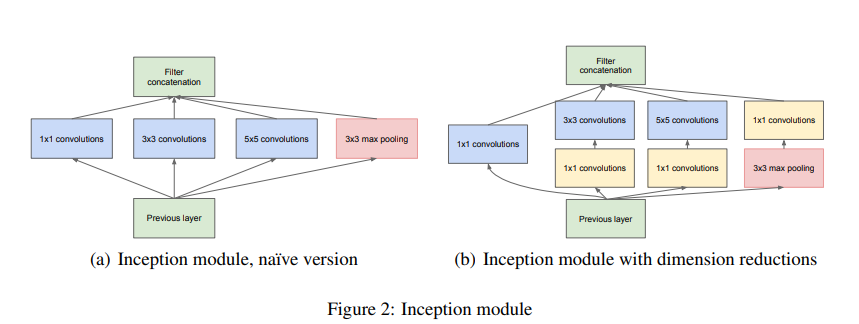
\includegraphics[width=1.0\columnwidth]{2.png}
\end{figure}

\subsection{Considere una aproximación clásica al reconocimiento de escenas
en donde extraemos de la imagen un vector de características y lo
usamos para decidir la clase de cada imagen. Compare este
procedimiento con el uso de una CNN para el mismo problema. ¿Hay
conexión entre ambas aproximaciones? En caso afirmativo indique en
que parecen y en que son distintas.}

% DONE

La diferencia radica en la extracción de las características, con una CNN 
mediante las capas de convolución y activación se eligen las características
relevantes de la imagen de cara a su clasificación. \newline

Son las capas completamente conectadas y la función softmax las que clasifica la
imagen, y esto es independiente del método por el cuál se hayan obtenido las
características.

\newpage

\subsection{¿Cómo evoluciona el campo receptivo de las neuronas de una CNN
con la profundidad de la capas?\newline ¿Se solapan los campos receptivos de
las distintas neuronas de una misma profundidad?\newline ¿Es este hecho algo
positivo o negativo de cara a un mejor funcionamiento?}

% DONE

El campo receptivo cada vez se agranda más, pues va recogiendo información de 
múltiples neuronas inferiores (siendo estas más específicas). Esto hace que con el 
tiempo se utilice información de regiones más grandes de la imagen. \newline

Por el funcionamiento de la convolución, salvo excepciones (por ejemplo, que se 
aumente el stride) las neuronas solapan sus campos receptivos. \newline

Puesto que la convolución captura información espacial de la imagen, y
siendo claro que píxeles cercanos aportan cierta información local sobre esta, el hecho
de que los campos receptivos se solapen refuerza a que un píxel comparta esta
información junto a sus cercanos y no sea separado en una zona u otra en función
de la máscara que se haya utilizado. \newline 

Si cayese en una región donde predomine otro
tipo de información, el píxel pierde relevancia y acaba no teniendo repercusión.
Al solaparse los campos receptivos, puede reforzar la información de varias regiones.

\subsection{¿Qué operación es central en el proceso de aprendizaje y
optimización de una CNN?}

% DONE

La más importante para cualquier tipo de red neuroral es el algoritmo de 
backpropagation, ya que es la que ajusta los pesos de las neuronas con el 
objetivo de bajar el error. \newline

Si especificamos en CNN, la convolución es la operación principal que permite
obtener características de la imagen. Es necesario tratar con cuidado sus
hiperparámetros (tamaño de máscara, dimensión de salida, stride...) para evitar
generar un gran coste computacional en la red.

\subsection{Compare los modelos de detección de objetos basados en
aproximaciones clásicas y los basados en CNN y diga que dos procesos
comunes a ambos aproximaciones han sido muy mejorados en los modelos
CNN. Indique cómo.}

% DONE

Ambos modelos proponen regiones sobre los que determinar si existe objeto
o no. Este proceso ha ido mejorando con el tiempo, mientras que antiguamente se
utilizaba una ventana deslizante para seleccionar estas regiones, los modelos
modernos se centran en elegir de mejor manera un conjunto de bounding-boxes de 
menor tamaño y en ocasiones aprendible por la NN. \newline

La comprobación de si existe objeto o no en la región propuesta es el otro 
proceso mejorado con el paso del tiempo, mientras que antes se utilizaba HOG
como pattern matching para comprobar, ahora las CNN aprenden a detectar el objeto en
la región.

\subsection{Es posible construir arquitecturas CNN que sean independientes
de las dimensiones de la imagen de entrada. En caso afirmativo diga
cómo hacerlo y cómo interpretar la salida.}

% DONE

Es posible, pero hay que cambiar el tamaño de las imágenes
a la entrada de la red para ajustarlos a las dimensiones necesarias de las 
convoluciones de la primera capa. \newline

Esto se puede hacer por ejemplo con capas de Pooling, seleccionando en localmente
los píxeles más relevantes mientras se reduce dimensionalidad. \newline

Es necesario tener en cuenta que detalles relevantes a la clasificación de la
imagen pueden haberse perdido con estas operaciones.

\subsection{Suponga que entrenamos una arquitectura Lenet-5 para clasificar
imágenes 128x128 de 5 clases distintas.\newline Diga que cambios deberían de
hacerse en la arquitectura del modelo para que se capaz de detectar
las zonas de la imagen donde aparecen alguno de los objetos con los
que fue entrenada.}

% DONE

Es necesario hacer que la red aprenda las coordenadas del objeto que detecta,
preferiblemente regiones simples (como un rectángulo) de cara a la optimización. \newline

Para ello se deriva la salida de la red previa a su clasificador hacia uno nuevo
en el que se evalue el ground truth del objeto, y la función de pérdida calculada
se junte con la del clasificador de Lenet para crear una sola. Una vez juntadas,
se puede realizar backpropagation para entrenarla como una red única.

\subsection{Argumente por qué la transformación de un tensor de dimensiones
128x32x32 en otro de dimensiones 256x16x16, usando una convolución
3x3 con stride=2, tiene sentido que pueda ser aproximada por una
secuencia de tres convoluciones: convolución 1x1 + convolución 3x3
+ convoluión 1x1.\newline Diga también qué papel juegan cada una de las tres
convoluciones.}

% DONE

Las convoluciones 1x1 solo juegan con el tamaño del tensor.
De esta manera se consigue optimizar los cálculos de la capa, combinando 
características de los diferentes canales. \newline

En este caso, tenemos que:
\begin{itemize}
	\item La primera convolución 1x1 es para reducir dimensionalidad y hacer la 
	3x3 más rápida.
	\item La 3x3 es la convolución con stride en sí, reduciendo de 32x32 a 16x16.
	\item La última aumenta al número de canales deseado, en este ejemplo 256.
\end{itemize}

No es la misma transformación pues se reduce la profundidad del tensor con la
primera convolución, pero se asume que la información espacial está distribuida
a través de un canal, y no entre los canales en sí. Con esta suposición podemos 
dejar a la convolución a que aprenda a reducir las dimensiones de manera que se aproveche la
máxima información posible.

\newpage 

\subsection{Identifique una propiedad técnica de los modelos CNN que permite
pensar que podrían llegar a aproximar con precisión las
características del modelo de visión humano, y que sin ella eso no
sería posible.\newline Explique bien su argumento.}

% DONE

Según mostraron Hubel y Wiesel, las células del córtex humano se estructuran en 
una jerarquía ascendente, compuesta de:
\begin{itemize}
	\item Células simples, que responden a bordes en zonas específicas del campo visual.
	\item Células complejas, que responden a bordes en zonas más grandes del campo visual.
	\item Células hipercomplejas, que responden a diferentes combinaciones de 
	características.
\end{itemize}

\begin{figure}[h]
	\centering
	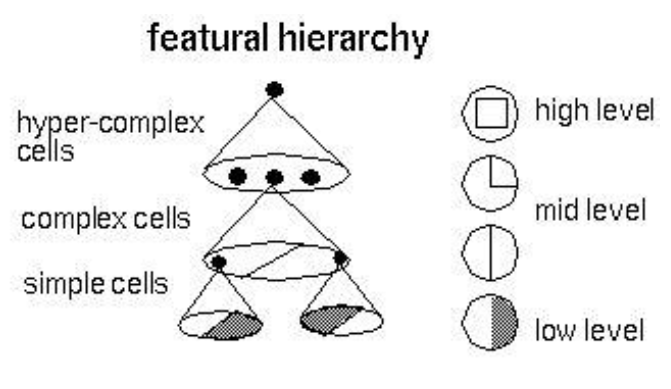
\includegraphics[width=1.0\columnwidth]{1.png}
\end{figure}

Esta división da a entender que las neuronas trabajan con características
locales de la visión y utilizan información de las neuronas inferiores.
Además, células contiguas representan zonas cercanas del campo visual. \newline

Las CNN se basan en esa misma ideología y por ello es posible pensar en alcanzar
el potencial humano. 
Pero puesto que no se sabe a ciencia cierta que tipo de operaciones realizan
las neuronas del córtex no podemos saber si las CNN podrán llegar a simular el 
funcionamiento. \newline

Esto no implica que no sea posible alcanzar los mismos niveles de precisión, se
ha visto que con el potencial de las CNN se pueden alcanzar rendimientos muy buenos.

\end{document}
